%************************************************
\chapter{Equazioni conservative del moto}\label{chp:ConservazioneMoto}
%************************************************
Esistono due approcci alla descrizione del moto di un fluido all'interno di un determinato volume:
\begin{itemize}
\item Approccio Lagrangiano
\item Approccio Euleriano
\end{itemize}
\paragraph{Approccio Lagrangiano}
La descrizione lagrangiana di un flusso di un fluido traccia la posizione delle singole particelle dello stesso.
Il flusso può essere pensato come la composizione di un un numero finito di particelle di fluido che hanno: massa, momento, energia inerziale e altre proprietà. Dunque si può descrivere lo stato delle singole particelle a partire da equazioni per ognuna.
Ciò rende difficile sfruttare questo metodo per un'analisi pratica:
\begin{enumerate}
\item I fluidi sono composti da miliardi di molecole (particelle);
\item le interazioni tra le molecole sono difficili da descrivere analiticamente.
\end{enumerate} 
Questo approccio viene comunque usato in alcuni campi come: dinamica di spray, bolle e particelle; per l'accoppiamento dei metodi euleriani-lagrangiani.

\paragraph{Approccio Euleriano}
la descrizione euleriana di un fluido, viene definito un volume di controllo in cui il fluido scorre all'interno.
Si considera come le proprietà del fluido cambiano nel volume di controllo, che viene fissato nello spazio e nel tempo. Invece che seguire le singole particelle nello spazio.
Viene definito uno spazio di variabili che sono funzioni dello spazio e del tempo come:
\begin{description}
\item[Campo di velocità] $\textbf{V} = \textbf{V}(x, y, z, t)$
\item[Campo di pressione] $p = p(x, y, z, t)$
\item[Campo di densità] $\rho = \rho(x, y, z, t)$
\item[Campo di temperatura] $T = T(x, y, z, t)$
\item[\dots]
\end{description}
Resta necessario imporre una serie di condizioni di contorno affinché il sistema possa essere ben definito.

Alla figura \ref{fig:ModelliLagEul} vengono rappresentati i due modelli.

\begin{figure}
\centering
\subfloat[][\emph{Modello lagrangiano}\label{fig:Lagrangiano}]
{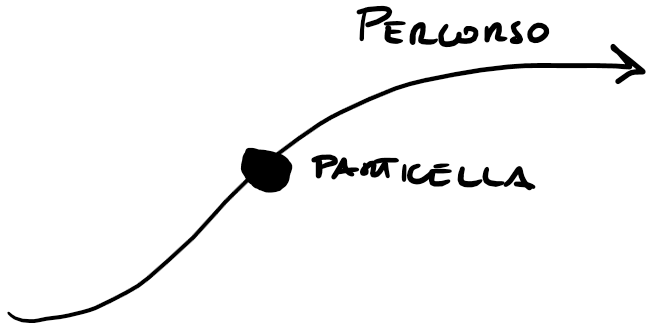
\includegraphics[width = 0.4\textwidth]{gfx/Lagrangiano}}\quad
\subfloat[][\emph{Modello Euleriano}\label{fig:Euleriano}]
{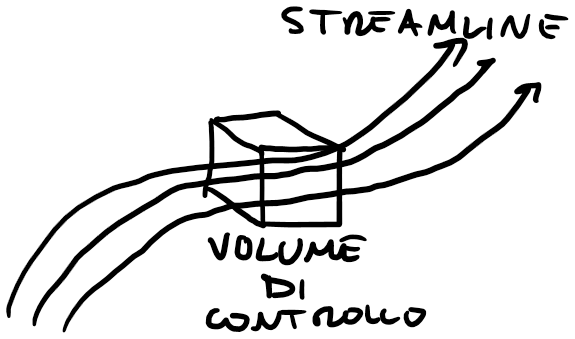
\includegraphics[width = 0.4\textwidth]{gfx/Euleriano}}
\caption{Esempi dei modelli di Lagrange ed Eulero}
\label{fig:ModelliLagEul}
\end{figure}

\section{Particelle di un fluido}
Il comportamento di un fluido è definito in termini macroscopici da%
\footnote{Vengono ignorate le notazioni $(x, y, z, t)$ per comodità, si ricorda che sono tutte funzioni di questi parametri.}
:
\begin{itemize}
\item Velocità $\textbf{u}$
\item Pressione $p$
\item Densità $\rho$
\item Temperatura $T$
\item Energia (cinetica) $E$, Entalpia $H$
\end{itemize}
Le proprietà risultano medie nel caso si considerino un numero sufficiente di particelle.
Un elemento fluido può essere pensato come il più piccolo volume per il quale la condizione di continuità è comunque valida.

\subsection{Derivate totali}
Considerando un fluido arbitrario, per una particella in moto nel fluido, questa sperimenta:
\begin{enumerate}
\item un cambiamento del fluido in funzione del tempo;
\item cambiamenti in base al fatto che più particelle si muovono in diverse direzioni nel fluido con diverse condizioni.
\end{enumerate}
La somma di queste due, per una caratteristica per unità di massa è chiamata come la derivata totale:
\begin{equation}
\frac{D\phi}{Dt} = \frac{\partial \phi}{\partial t} + V_x \frac{\partial \phi}{\partial x} + V_y \frac{\partial \phi}{\partial y} + V_z \frac{\partial \phi}{\partial z} = \frac{\partial \phi}{\partial t} + (\textbf{V} \cdot \nabla)\phi
\label{eqn:DerivataTotale}
\end{equation}
L'operatore \textbf{derivata totale}, $D/Dt$, fornisce la trasformazione tra il modello lagrangiano e quello euleriano.

Considerando l'accelerazione del fluido, può essere definita come:
\begin{equation}
\frac{D\mathbf{V}}{Dt} = \frac{\partial \mathbf{V}}{\partial t} + (\mathbf{V}\cdot \nabla) \mathbf{V}
\label{eqn:Accelerazione}
\end{equation}

dove:\\
\begin{tabular}{cl}
$\frac{\partial}{\partial t}$ & Derivata locale\\
$(\mathbf{V} \cdot \nabla) \mathbf{V}$ & Derivata di convezione\\
\end{tabular}\\

La derivata locale è diversa da zero solamente nel caso di flussi stazionari.
Mentre, la derivate di convezione è principalmente dovuta al fatto che le particelle sono in movimento.

Dunque, se la velocità del fluido è costante allora: l'accelerazione locale è nulla, allo stesso modo, l'accelerazione di convezione è sempre diversa da zero perché la particella si muove in altre posizioni caratterizzata dalla diversa velocità nel fluido.

Prendiamo come esempio il caso del flusso d'acqua dall'ugello, rappresentato in figura \ref{fig:EsempioAcqua}. 
Consideriamo per esempio l'approccio Euleriano sotto le seguenti ipotesi:
il flusso è stazionario nel caso in cui tutte le proprietà del flusso non cambiano in funzione del tempo.

\begin{figure}
\centering
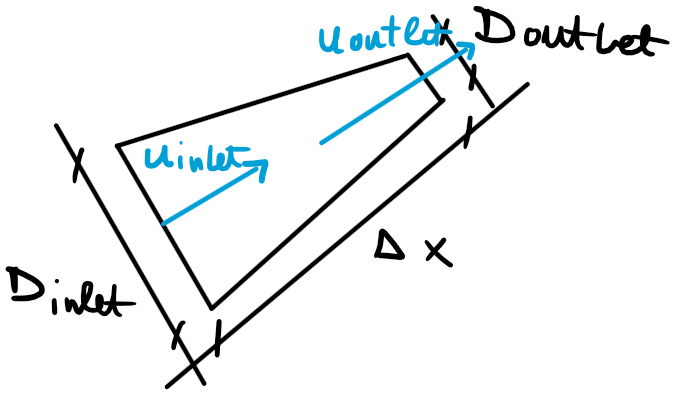
\includegraphics[width = 0.7\textwidth]{gfx/EsempioAcqua}
\caption{Esempio dell'ugello della canna dell'acqua}
\label{fig:EsempioAcqua}	
\end{figure}

Vale che la velocità all'uscita dell'ugello è più grande rispetto a quella di ingresso.
Perciò, il fluido deve accelerare all'interno del volume, anche se si è sotto l'ipotesi di stazionarietà.
Qui entra in gioco la derivata di convezione, questo parametro sarà sicuramente non nullo da cui i fenomeni di accelerazione.

Si evince che: secondo il modello euleriano, il sistema risulta stazionario. se invece si trasporta il tutto nel modello lagrangiano, ne risulta un'accelerazione delle particelle che entrano ad una data velocità ma escono ad una superiore.

\section{Conservazione della massa}
\begin{equation}
\frac{\partial \rho}{\partial t} + \nabla \cdot (\rho\mathbf{V}) = 0
\label{eqn:EquazioneConservazione}
\end{equation}

\begin{quote}
\emph{Il flusso in entrata e in uscita da un determinato volume varia al variare della massa compresa all'interno dello stesso volume di controllo.}
\end{quote}

\subsection{Funzione di flusso}
Le linee di corrente o \textbf{\eng{Streamlines}} soddisfano l'equazione di continuità e rappresentano su un piano cartesiano la funzione di flusso.

prendiamo il caso di un fluido bidimensionale incomprimibile sul piano x-y%
\footnote{$V_z = 0$ sia $V_x$ che $V_y$ non dipendono dalle componenti in $z$}.
L'equazione di continuità viene ridotta a $\frac{\partial V_x}{\partial x} + \frac{\partial V_y}{\partial y} = 0$.
La trasformazione di una variabile ci permette di riscrivere l'equazione in termini dipendenti da una sola variabile: la \textbf{funzione di flusso $\Psi$}:
\graffito{Il significato fisico della funzione $\Psi$ è che le curve della costante rappresentano le \eng{streamlines} del flusso.}
\begin{equation}
V_x = \frac{\partial \Psi}{\partial y} \qquad V_y = \frac{\partial \Psi}{\partial x}
\label{eqn:CambioVar}
\end{equation} 
Sostituendo nell'equazione di continuità:
\begin{equation}
\frac{\partial^2 \Psi}{\partial x \partial y} - \frac{\partial^2 \Psi}{\partial x \partial y} = 0
\label{eqn:StreamFunction}
\end{equation}

\begin{figure}
\centering
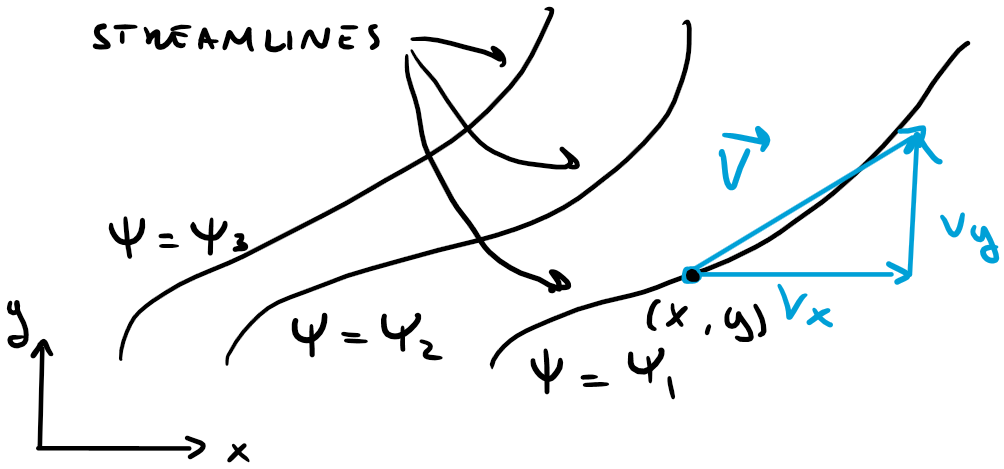
\includegraphics[width = \textwidth]{gfx/Streamlines}
\caption{Rappresentazione delle \eng{streamlines}}
\label{fig:Streamlines}
\end{figure}

Un'ulteriore considerazione deriva dal fatto che seguendo le ipotesi di:
\begin{itemize}
\item si assume che un fluido possa essere rapresentato tramite \eng{streamlines};
\item valga comunque la similitudine dei triangoli;
\end{itemize}
Allora si dimostra che:\\
\textit{La \eng{streamline} è una curva che è sempre istantaneamente tangente al vettore velocità locale}.

A partire dalla similitudine dei triangoli vale che (Vedi figura \ref{fig:Streamlines}):
\begin{equation}
\frac{dr}{V} = \frac{dx}{V_x} = \frac{dy}{V_y}
\label{eqn:SimTriangoli}
\end{equation}
Dalla \eqref{eqn:SimTriangoli} vale: $V_x dy = V_y dx$.
Sostituendo con la definizione della \eqref{eqn:CambioVar}, può essere scritta la:
\begin{equation}
\frac{\partial \Psi}{\partial y} dy + \frac{\partial \Psi}{\partial x} dx = 0
\end{equation}
Allora la variazione totale di $\Psi$ (in uno spazio infinitesimale $x+dx, y+dy$) vale%
\footnote{Si ricorda che la somma delle derivate parziali fatte rispetto alle variabili indipendenti è la derivata totale.}:
\begin{equation}
\frac{\partial \Psi}{\partial y} dy + \frac{\partial \Psi}{\partial x} dx = d\Psi
\end{equation}
Da cui deve essere che 
\begin{equation}
d\Psi = 0
\end{equation}
Questo significa che $\Psi = cost.$ lungo le \eng{streamlines}.

\graffito{Il significato fisico di questa affermazione è che: \textit{la differenza del valore di $\Psi$ tra due \eng{streamlines} è uguale al flusso di volume per la distanza tra le due linee}.}
Siccome, per definizione, alcun flusso può attraversare una \eng{streamline}, il fluido reste confinato tra le due stesse.
Ne segue che, per un flusso stazionario e incomprimibile bidimensionale, il flusso di volume $\dot{V}$ per unità di tempo tra due \eng{streamlines} deve essere costante (per garantire la validità dell'equazione di continuità).
Se due \eng{streamlines} si separano, la velocità media del flusso calerà uniformemente.

Analogamente a quanto visto fin ora, ovvero una descrizione delle \eng{streamlines} in coordinate cartesiane; la trattazione è del tutto equivalente per un sistema di riferimento in coordinate cilindriche.
A partire dalle stesse ipotesi, l'equazione di continuità può essere descritta come:
\begin{equation}
\frac{\partial (r V_r)}{\partial r} + \frac{\partial V_{\theta}}{\partial \theta} = 0
\end{equation}
Ora, la funzione di continuità viene comunque soddisfatta da una qualsiasi legge continua $\Psi = \Psi(r,\theta)$ dato che l'ordine di differenziazione è irrilevante.
Allora, per un fluido incomprimibile assisimmetrico (c'è simmetria nella rotazione dell'asse $z$) in assenza di vortici%
\footnote{$V_{\theta} = 0$ né $V_r$ né $V_z$ dipendono da $\theta$}, la funzione di continuità può essere descritta come
\begin{equation}
\frac{1}{r}\frac{\partial r V_r}{\partial r} + \frac{\partial V_z}{\partial z}  = 0
\end{equation}

\paragraph{Considerazioni}
Al di là della definizione di \eng{streamline} in qualsiasi sistema di riferimento, grazie all'osservazione di queste si può tracciare le linee di corrente soddisfacenti la conservazione della massa, permettendo di descrivere l'andamento del flusso all'interno del volume.
Vale anche:
\begin{description}
\item[\eng{streamlines} divergenti] $\Rightarrow$ velocità di flusso minore $\Rightarrow$ decelerazione delle particelle o flusso.
\item[\eng{streamlines} convergenti] $\Rightarrow$ Velocità di flusso maggiore $\Rightarrow$ accelerazione delle particelle o flusso.
\end{description}

\section{Conservazione del momento}
Per la trattazione della conservazione del momento da parte delle particelle di un fluido è necessario introdurre l'\textbf{equazione di Cauchy}.

\subsection{Equazione di Cauchy}
\begin{equation}
\rho \frac{D\mathbf{V}}{Dt} = \rho \mathbf{g} + \nabla \cdot \boldsymbol{\sigma}
\label{eqn:Cauchy}
\end{equation}
Dove viene definito $\boldsymbol{\sigma}$ come \textbf{Cauchy stress tensor}:
\begin{equation}
\boldsymbol{\sigma} = -p\mathbf{I} + \boldsymbol{\tau}
\label{eqn:StressTensorCauchy}
\end{equation}
Che scritto in forma matriciale diventa:
\begin{equation}
\underbrace{%
\begin{bmatrix}
\sigma_{xx} & \sigma_{xy} & \sigma_{xy} \\
\sigma_{yx} & \sigma_{yy} & \sigma_{yz} \\
\sigma_{zx} & \sigma_{zy} & \sigma_{zz}
\end{bmatrix}}_{= \boldsymbol{\sigma}} =%
\underbrace{%
\begin{bmatrix}
-p & 0 & 0 \\
0 & -p & 0 \\
0 & 0 & -p
\end{bmatrix}}_{\text{parte isotropa di } \boldsymbol{\sigma}} +%
\underbrace{%
\begin{bmatrix}
\tau_{xx} & \tau_{xy} & \tau_{xz} \\
\tau_{yx} & \tau_{yy} & \tau_{yz} \\
\tau_{zx} & \tau_{zy} & \tau_{zz} 
\end{bmatrix}}_{\text{parte anisotropa di} \boldsymbol{\sigma}}
\label{eqn:StressTensorCauchyMatrix}
\end{equation}
Per un fluido a riposo, l'unico sforzo in un elemento del fluido è la pressione idrostatica locale, la quale agisce uniformemente normale a qualsiasi superficie del fluido (componente isotropa di $\boldsymbol{\sigma}$).
Mentre, per un fluido in movimento, agisce comunque la componente isotropa. In più si aggiunge l'effetto dello sforzo viscoso $\boldsymbol{\tau}$ (componente anisotropa di $\boldsymbol{\sigma}$).
Tra l'altro, resta valido il fatto che lo sforzo viscoso è un effetto interno del fluido e non sulla superficie di controllo come accade per la componente isotropa.

Ora è necessario andare a descrivere che comportamento i fluidi abbiano in termini di componente anisotropa. Si rende necessario dividere i fluidi in base alla legge caratteristica di questo comportamento ovvero:
\begin{itemize}
\item fluidi newtoniani
\item fluidi non newtoniani
\end{itemize}

\subsubsection{Fluidi newtoniani}
I fluidi newtoniani sono tutti quei fluidi in cui lo sforzo viscoso è linearmente proporzionale alla deformazione del fluido.
In parole povere:
\begin{equation}
\boldsymbol{\tau} \propto \boldsymbol{\epsilon}
\end{equation}
Possiamo definire che la proporzionalità, assumendo che valga l'ipotesi di Stokes%
\footnote{Ovvero che il comportamento del fluido sia comparabile lungo i tre assi principali}:
\begin{equation}
\boldsymbol{\tau} = 2 \mu \boldsymbol{\epsilon} - \frac{2}{3} \mu \nabla \cdot \mathbf{V}
\label{eqn:NewtFluid}
\end{equation}
Nell'equazione \eqref{eqn:NewtFluid} viene aggiunto il parametro $\mu$ il quale indica la viscosità dinamica. Spesso si può trovare anche sotto forma di $\nu$ definito come $\nu = \mu / \rho$.
Si può legare la viscosità dinamica, in entrambe le sue forme, come: $\mu = f(T,p)$ ovvero che la viscosità dinamica dipende sia dalla temperatura che dalla pressione.
In particolare, si può dimostrare come dipenda fortemente dalle variazioni di temperatura e debolmente da quelle di pressione.
Resta importante capire che la viscosità dinamica è un fenomeno interno al fluido, qualunque esso sia, infatti si tratta della frizione tra i vari substrati del fluido.

\subsubsection{Fluidi non newtoniani}
Per questi fluidi non si può considerare la viscosità come costante, ma potrebbe variare in funzione dello sforzo.
Riprendendo i termini dell'equazione di Cauchy \eqref{eqn:StressTensorCauchy}:
\begin{equation}
\boldsymbol{\sigma} = \mu \dot{\gamma}
\label{eqn:NonNewtFluid}
\end{equation} 

\subsection{Equazione di Navier-Sockes}
\begin{equation}
\rho \frac{D\mathbf{V}}{Dt} = \rho \mathbf{g} - \nabla p + \mu \nabla^2\mathbf{V} + \frac{\mu}{3}\nabla(\nabla \cdot \mathbf{V})
\label{eqn:NavierStockes} 
\end{equation}
La quale può essere semplificata nel caso sussistano determinate condizioni:
\begin{description}
\item[Fluido incomprimibile] $(\nabla \cdot \mathbf{V}) = 0 $ allora l'equazione diventa:
\begin{equation}
\rho \frac{D\mathbf{V}}{Dt} = \rho \mathbf{g} - \nabla p + \mu \nabla^2\mathbf{V}
\end{equation}
\item[Fluido non viscido] si semplifica fino a (Equazione di Eulero):
\begin{equation}
\rho \frac{D\mathbf{V}}{Dt} = \rho \mathbf{g} - \nabla p
\label{eqn:Eulero}
\end{equation}
\end{description}
Si definisce un fluido non viscido nel momento in cui le forze viscose sono trascurabili rispetto alle forze d'inerzia, gravitazionali e di pressione.
Ad esempio lo sono le zone del fluido ad alto numero di \eng{Reynolds}.

I termini viscosi non sono trascurabili rispetto a quelli di inerzia nello strato limite in prossimità di un corpo immerso nel fluido. Ciò è dovuto ai forti gradienti di velocità presenti nello strato.

\paragraph{Fluido incomprimibile}
\begin{equation}
\rho \frac{D\mathbf{V}}{Dt} = \rho \mathbf{g} - \nabla p + \mu \nabla^2\mathbf{V}
\end{equation}
Si nota che il termine di pressione appare solo in forma di gradiente:
\begin{quote}
\textit{Il campo di velocità in un fluido incomprimibile non è affetto dalla pressione assoluta, bensì solo dalle differenze di pressione.}
\end{quote}
Eventuali modifiche alla pressione assoluta devono essere poste come condizioni al contorno del sistema.

Si può calcolare il campo di pressione con una costante arbitraria, ma per ottenere quella costante bisogna sapere il valore della pressione in qualche punto del fluido.
In altre parole, bisogna conoscere la pressione assoluta o totale come condizione al contorno.

Tutto ciò resta valido fin tanto che il fluido è incomprimibile, per fluidi comprimibili la pressione $p$ non è la pressione meccanica (forza/area) ma la pressione termodinamica $P$. In questo caso la pressione è funzione della temperatura e densità nell'equazione di stato del fluido.

\paragraph{Flusso Euleriano}
\begin{equation}
\rho \frac{D\mathbf{V}}{Dt} = \rho \mathbf{g} - \nabla p + \mu \nabla^2\mathbf{V}
\end{equation}
In questo caso esistono delle regioni non viscide del fluido che possono essere trascurate per la maggior parte del fluido. Non devono essere ignorate sempre.
Dato ciò si può assumere:
\begin{equation}
\underbrace{\tau}_{\text{sforzo viscoso}} \approx \underbrace{\mu}_{\text{viscosità}} \times \underbrace{\frac{\partial V_i}{\partial x_i}}_{\text{gradiente di velocità}}
\end{equation}
\begin{quote}
\textit{I termini viscosi non sono trascurabili in presenza di forti variazioni del gradiente di velocità (strato limite, scia del corpo, \dots).}
\end{quote}

La figura \ref{fig:EulerianEquation} mostra un caso dove può essere applicata l'equazione di Eulero e dove no.

\begin{figure}
\centering
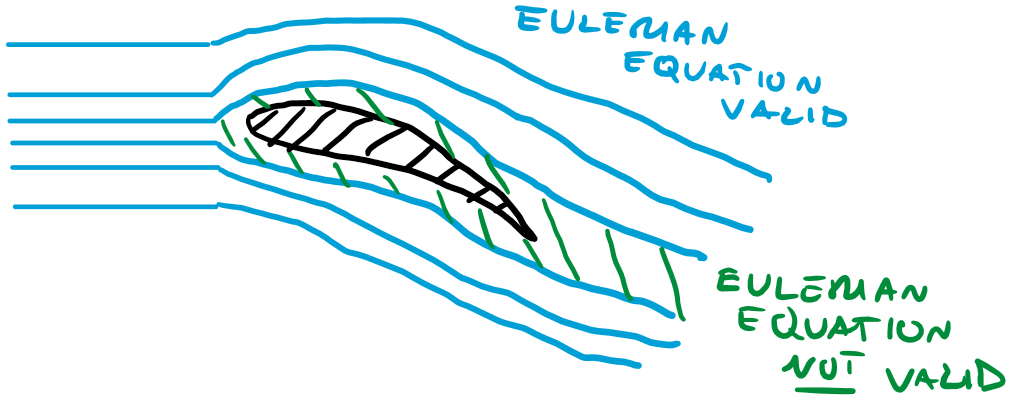
\includegraphics[width = 0.7\textwidth]{gfx/EulerianEquation}
\caption{Osservazione dove l'equazione di Eulero è valida e non.}
\label{fig:EulerianEquation}
\end{figure}

\subsection{Equazione di Bernoulli}
La somma della pressione, dell'energia cinetica e potenziale delle particelle di un fluido è costante lungo la \eng{streamline} nel caso di un flusso stazionario quando i termini di comprimibilità e viscosità sono trascurabili:
\begin{equation}
\frac{p}{\rho} + \frac{V^2}{2}+gz = cost.
\label{eqn:Bernoulli}
\end{equation}
Da notare che la costante di Bernoulli può cambiare tra diverse \eng{streamlines} ma è costante nella singola.
Nel flusso stazionario incomprimibile con effetti viscosi trascurabili, le varie forme di energia vengono trasformate ma la loro somma resta costante. Non c'è dissipazione di energia meccanica lungo il flusso.
L'equazione di Bernoulli è una relazione approssimativa tra pressione, velocità ed elevazione; resta valida solamente nelle regioni non viscide del fluido.

\paragraph{Pressione modificata}
Gli effetti della gravità sono rilevanti solamente su flussi a superficie libera: ad esempio onde, moto di una nave. e per flussi guidati dalle condizioni a contorno come il moto per convezione naturale.

Per flussi incomprimibili, senza superfici libere, la gravità non modifica la dinamica del flusso. Il suo effetto sarà di imporre una pressione idrostatica distribuita nella direzione verticale rispetto al campo di pressione del fluido.
Si può definire una pressione modificata $p'$ che assorbe l'effetto della pressione idrostatica apportata dalla gravità. In questo caso, con l'asse $z$ diretto in opposizione rispetto a $\mathbf{g}$ e, definito un riferimento nullo sull'asse $z$ allora:
\begin{equation}
p' = p + \rho g z \Rightarrow \rho \frac{D\mathbf{V}}{Dt} = \nabla p' + \mu \nabla^2\mathbf{V}
\end{equation}
Il vantaggio di calcolare secondo l'equazione di Navier-Stockes è che non include il termine gravitazionale. Dopo la risoluzione con quella equazione, in termini di $p'$ è semplice tornare alla pressione senza contributo idrostatico $p = p' - \rho g z$

La pressione modificata è spesso usata nelle analisi \ac{CFD} per separare gli effetti gravitazionali da quelli del fluido.
La pressione modificata non deve essere usata in flussi con superfici libere.

\section{Conservazione dell'energia}
Per analizzare iun fluido in termini energetici conviene visualizzare l'equazione dell'entalpia totale.

\subsection{Equazione dell'entalpia totale}
\begin{equation}
\rho \frac{Dh_0}{Dt} = \rho \mathbf{g} \cdot \mathbf{V} + \frac{\partial p}{\partial t} + \nabla \cdot (k \nabla T) + q_g + \nabla \cdot (\boldsymbol{\tau} \cdot \mathbf{V})
\label{eqn:TotalEnthalpy}
\end{equation}
Dove:\\
\begin{tabular}{cl}
$q_g$ & rappresenta il calore generato internamente dal sistema\\
$\nabla \cdot (\boldsymbol{\tau} \cdot \mathbf{V})$ & rappresenta il lavoro fatto dallo sforzo viscoso
\end{tabular}\\
Da cui ne derivano:
\begin{description}
\item[Equazione dell'entalpia] da non confondere con quella totale
\begin{equation}
\rho \frac{Dh}{Dt} = \frac{Dp}{Dt} + \nabla \cdot (k \nabla T) + q_g + \underbrace{\boldsymbol{\tau} \cdot \nabla \mathbf{V}}_{= \Phi}
\end{equation}
\item[Equazione entropia]
\begin{equation}
\rho T \frac{Ds}{Dt} = \nabla \cdot (k \nabla T) + q_g + \underbrace{\boldsymbol{\tau} \cdot \nabla \mathbf{V}}_{= \Phi}
\end{equation}
\end{description}
La dissipazione dovuta agli attriti viscosi $\Psi$ rappresenta l'ammontare del lavoro fatto dagli sforzi viscosi. Il quale viene convertito in calore il quale processo è irreversibile. Da cui una fonte di calore irreversibile.
L'effetto della dissipazione viscosa nello scambio termico è particolarmente significativa per fluidi ad alta velocità e altamente viscosi. 

Dalla \eqref{eqn:TotalEnthalpy} i parametri sono indicati come:\\
\begin{tabular}{cp{0.8\textwidth}}
$\rho \mathbf{g} \cdot \mathbf{V}$ & Lavoro fatto dalle forse del corpo\\
$\frac{\partial p}{\partial t}$ & Influenza della pressione nell'entalpia totale\\
$\nabla \cdot (k\nabla T)$ & Quantità di energia trasferita per conduzione dal corpo al volume di controllo\\
$q_g$ & Calore generato da una fonte interna\\
$\nabla \cdot (\boldsymbol{\tau} \cdot \mathbf{V})$ & Lavoro degli effetti viscosi 
\end{tabular}

Da cui si può ricavare l'equazione dell'entalpia statica.

\subsection{Equazione dell'entalpia statica}
\begin{equation}
\rho \frac{Dh}{Dt} = \frac{Dp}{Dt} + \nabla \cdot (k \nabla T) + q_g + \boldsymbol{\tau} \cdot \nabla \mathbf{V}
\label{eqn:StaticEnthalpy}
\end{equation}
L'equazione data come entalpia totale descrive i cambiamenti, in termini termici e meccanici, dell'energia.
Il termine dinamico dell'entalpia totale \eqref{eqn:TotalEnthalpy} può essere sottratto e l'equazione \eqref{eqn:StaticEnthalpy} è descritta per ottenere un'equazione per valutare il cambiamento dei parametri termodinamici dell'energia termica e entalpia.
Sotto alcune ipotesi, può essere utilizzata per descrivere un fluido poco comprimibile, quando la comprimibilità del flusso è comunque bassa. 

\section{Equazioni di stato}
Il moto del fluido è descritto da cinque equazioni differenziali parziali per la descrizione della: massa, momento ed energia.
I parametri termodinamici da ricercare in queste equazioni sono: $\rho$, $p$, $h$ e $T$.
Assumeremo l'equilibrio termodinamico: ovvero che il tempo necessario alle particelle per adeguarsi a nuove condizioni di contorno sia corto rispetto alle caratteristiche temporali del fluido.
Dobbiamo aggiungere due equazioni di stato usando due variabili: $p = p(\rho, T)$, $h = h(p, T)$.

\subsection{Equazione di stato per un fluido incomprimibile}
\begin{equation}
\rho = cost.
\end{equation}
Valida per liquidi e buona approssimazione per gas a bassa velocità.

Si può assumere che il flusso sia incomprimibile a patto che la massima compressione sia al di sotto del $5\%$. Ciò implica che la velocità del gas sia inferiore al numero di Mach $ Ma \lesssim 0.3$
Non c'è collegamento tra l'equazione dell'energia e le equazioni di massa e momento. Si risolve l'equazione di energia solo in caso di trasferimento di calore.
Il campo di velocità non è affetto dal valore assoluto della pressione ma solo dal gradiente.
Per i flussi comprimibili, la pressione è legata con la densità e temperatura attraverso un'equazione di stato e allora il valore della pressione assoluta. Un flusso comprimibile richiede una soluzione non solo di massa e momento, anche di energia e un'equazione di stato.

\subsection{Equazione di stato del gas ideale}
\begin{equation}
p = \rho R T
\label{eqn:IdealGas}
\end{equation}
Il fattore di comprimibilità $Z = \frac{p}{\rho R T}$ la cui variazione da una buona misura dell'applicabilità dell'equazione \eqref{eqn:IdealGas}.

\subsection{Equazioni del gas reale}
Per descrivere l'andamento di un gas reale esistono diversi modelli, descritti nel tempo.
Hanno una forma simile a quella del gas ideale \eqref{eqn:IdealGas} ma con degli aggiustamenti ai coefficienti per poter modellizzare correttamente il funzionamento di uno specifico gas.
In letteratura si trovano articoli che descrivono quale modello rappresenta meglio un dato gas.

\section{Equazioni costitutive}
Alcuni parametri sono determinati da equazioni costitutive, in funzione di diversi parametri termodinamici.
Ad esempio la viscosità, dipende fortemente dalla temperatura.
Per diversi casi vengono definite le loro equazioni costitutive in modo che si possa determinare il valore del parametro per ogni caso.

\section{Condizioni al contorno}
In qualsiasi punto su un limite formato da una superficie solida impermeabile, la continuità richiede che la componente normale della velocità alla superficie sia la stessa per il fluido che per la superficie.
Se un limite solido è stazionario, quindi la posizione della superficie non cambia nel tempo e, definito $\mathbf{n}$ come normale alla superficie, allora:
\begin{equation}
\mathbf{u} \cdot \mathbf{n} = 0 
\end{equation}
sulla superficie.
Per una fluido reale e viscoso, c'è una condizione addizionale sulla velocità tangenziale alla superficie. La condizione alla superficie per un fluido viscoso è che non può esserci velocità tangenziale relativa tra la superficie e il fluido.

%%%%%%%%%%%%%%%%%%%%%%%%%%%%%%%%%%%%%%%%%%%%%%%%%%%%%%%%%%%%%%%%%%%%%%%%%%%%%%%
\chapter{Flussi rotazionali e irrotazionali}\label{chp:RotIrrotFlow}
%%%%%%%%%%%%%%%%%%%%%%%%%%%%%%%%%%%%%%%%%%%%%%%%%%%%%%%%%%%%%%%%%%%%%%%%%%%%%%%
\section{Tipologie, movimenti e deformazioni di elementi fluidi}
Un elemento di un fluido può essere sottoposto a quattro tipologie di movimento e deformazione:
\begin{enumerate}
\item traslazione
\item rotazione
\item sforzo lineare
\item sforzo di taglio
\end{enumerate}
Siccome abbiamo necessità di descrivere gli elementi in movimento allora le misure che più ci interessano sono (rispettivamente):
\begin{enumerate}
\item Velocità
\item velocità angolare
\item sforzo lineare
\item sforzo di taglio
\end{enumerate}
Con l'obbiettivo di calcolare le caratteristiche del fluido è necessario che questi parametri siano in funzione della velocità o delle sue derivate.
Per esempio:
\begin{description}
\item[Vettore velocità]
\begin{equation}
\mathbf{V} = V_x \mathbf{i} + V_y \mathbf{j} + V_z \mathbf{k}
\end{equation}
\item[Vettore velocità angolare]
\begin{equation}
\vec{\omega} = \omega_x \vec{i} + \omega_y \vec{j} + \omega_z \vec{z}\\
\end{equation}
\item[Stress lineare]
\begin{equation}
\epsilon_{xx} = \frac{\partial V_x}{\partial x} \quad \epsilon_{yy} = \frac{\partial V_y}{\partial y} \quad \epsilon_{zz} = \frac{\partial V_z}{\partial z}
\end{equation}
\item[Sforzo di taglio]
\begin{equation}
\epsilon_{xy} = \frac{1}{2}\left(\frac{\partial V_x}{\partial y} + \frac{\partial V_y}{\partial x}\right) \quad \epsilon_{xz} = \frac{1}{2}\left(\frac{\partial V_z}{\partial x} + \frac{\partial V_x}{\partial z}\right) \quad \epsilon_{yz} = \frac{1}{2}\left(\frac{\partial V_y}{\partial z} + \frac{\partial V_y}{\partial z}\right)
\end{equation}
\end{description}
Da cui è possibile ottenere la matrice dello sforzo totale, in coordinate cartesiane:
\begin{equation}
\vec{\epsilon} =%
\begin{bmatrix}
\epsilon_{xx} & \epsilon_{xy} & \epsilon_{xz}\\
\epsilon_{yx} & \epsilon_{yy} & \epsilon_{yz}\\
\epsilon_{zx} & \epsilon_{zy} & \epsilon_{zz}
\end{bmatrix}%
=%
\begin{bmatrix}
\frac{\partial V_x}{\partial x} & \frac{1}{2}\left(\frac{\partial V_x}{\partial y} + \frac{\partial V_y}{\partial x}\right) & \frac{1}{2}\left(\frac{\partial V_z}{\partial x} + \frac{\partial V_x}{\partial z}\right)\\
\frac{1}{2}\left(\frac{\partial V_x}{\partial y} + \frac{\partial V_y}{\partial x}\right) & \frac{\partial V_y}{\partial y} & \frac{1}{2}\left(\frac{\partial V_y}{\partial z} + \frac{\partial V_y}{\partial z}\right)\\
\frac{1}{2}\left(\frac{\partial V_z}{\partial x} + \frac{\partial V_x}{\partial z}\right) & \frac{1}{2}\left(\frac{\partial V_y}{\partial z} + \frac{\partial V_y}{\partial z}\right) & \frac{\partial V_z}{\partial z}
\end{bmatrix}
\end{equation}

\paragraph{Deformazione volumetrica}
Gli sforzi appena evidenziati non sono gli unici possibili per un fluido.
Ad esempio per diverse applicazioni è molto più importante la deformazione volumetrica.
Può essere espressa come:
\begin{equation}
\frac{1}{dN} \frac{D}{Dt} (dN) = \underbrace{\frac{\partial V_x}{\partial x} + \frac{\partial V_y}{\partial y} + \frac{\partial V_z}{\partial z}}_{= \nabla \cdot \vec{V}}
\end{equation}
Da cui si ricavano diverse casistiche:
\begin{description}
\item[Flusso incomprimibile] resta costante l'ammontare di volume netto: ciò indica che tanto si modifica il fluido in una direzione, tanto si deve stringere in altre direzioni per compensare.
\item[Flusso comprimibile] si modifica il parametro $dN$ in funzione dell'aumento o diminuzione della densità. 
\end{description}

\section{Vorticità e rotazionalità}
Si dice che un vettore è vorticoso nel caso: $\vec{\Omega} = \nabla \times \vec{V}$. Il rotore di una particella di dimostra essere doppia rispetto alla velocità di rotazione della stessa.
Il \textbf{rotore} è una misura dell'ammontare locale della rotazione del fluido.
Se $\vec{\Omega} \neq 0$ in una regione del fluido, allora le particelle stanno ruotando e il fluido in quella regione è detto rotazionale.
Se $\vec{\Omega} = 0$ 0 $\vec{\Omega} \approx 0$ allora la regione del fluido è detta irrotazionale.

La rotazione del fluido è spesso associata allo strato limite, scie, flusso attraverso turbomacchine e flusso con trasferimento di calore.

Il rotore di un fluido non può cambiare ameno di effetti della viscosità, gradienti di temperatura e altri fenomeni non-lineari.
Se un fluido origina in una regione irrotazionale, questo rimarrà irrotazionale fin tanto che qualche fenomeno non-uniforme ne altererà il comportamento.

Se una ragione del fluido può essere considerata come irrotazionale (o è molto vicina ad esserlo) le equazioni di moto si semplificano notevolmente. Una regione irrotazionale la pressione e forze di inerzia sono più importanti di quelle per effetti viscosi (ordini di grandezze più alte).

\section{Approssimazione a fluido irrotazionale}
L'approssimazione che una regione di fluido sia irrotazionale può andare bene per alcune regioni e non per altre.
In generale, regioni non viscide del flusso distanti da pareti solide e scie di altri corpi, sono considerabili irrotazionali; anche se ci sono delle situazioni per cui una regione non viscida potrebbe essere rotazionale.
Riprendendo l'esempio della figura \ref{fig:EulerianEquation} a pagina \pageref{fig:EulerianEquation}, le regioni lontane dal profilo alare possono essere considerate come irrotazionali. Strato limite e scia sono, invece, rotazionali.
Nelle regioni di flusso irrotazionali il vettore velocità può essere descritto come gradiente di una funzione scalare detta \textbf{velocità potenziale}.
\begin{equation}
\vec{V} = \nabla \phi
\end{equation}
resta valido:
\begin{equation}
\vec{\Omega} = \nabla \times \vec{V} \Rightarrow \nabla \times \nabla \phi = 0
\end{equation}
Le regioni irrotazionali sono anche dette regioni a flusso potenziale.

\subsection{Equazione di Laplace}
In coordinate cartesiane:
\begin{equation}
V_x = \frac{\partial \phi}{\partial x} \quad V_y = \frac{\partial \phi}{\partial y} \quad V_z = \frac{\partial \phi}{\partial z}
\end{equation}
In coordinate cilindriche:
\begin{equation}
V_r = \frac{\partial \phi}{\partial r} \quad V_{\theta} = \frac{\partial \phi}{\partial \theta} \quad V_z = \frac{\partial \phi}{\partial z}
\end{equation}
Che per un flusso incomprimibile e irrotazionale la velocità potenziale soddisfa l'equazione di Laplace ($\phi$ è una funzione armonica): 
\begin{equation}
\nabla^2\phi = 0
\end{equation}
Portata nelle coordinate cartesiane:
\begin{equation}
\frac{\partial^2 \phi}{\partial x^2} + \frac{\partial^2 \phi}{\partial y^2} + \frac{\partial^2 \phi}{\partial z^2} = 0 
\end{equation}
Le soluzioni dell'equazione di Laplace sono dominate dalla geometria (ad esempio condizioni al contorno) ì. Le tre componenti del vettore velocità sono combinati in una singola variabile $\phi$. Il problema è caratterizzato solamente da due variabili: $\phi$ e $p$.

\paragraph{Riassumendo:}
L'equazione di Laplace è fprtemente caratterizzata dalla geometria e:
\begin{itemize}
\item La conservazione della massa è sempre soddisfatta
\item Non c'è dipendenza dal tempo
\end{itemize}
Perciò: l'equazione è rappresentativa dei fenomeni transitori e la soluzione ottenuta tramite l'equazione è legata solamente alla condizione al contorno.

Dunque: per flussi incomprimibili e irrotazionali, la soluzione deve soddisfare solamente la condizione al contorno.

\subsection{Equazione di Eulero}
Riprendendo l'equazione di Navier-Stockes \eqref{eqn:NavierStockes} ridotta alle condizioni di incomprimibilità e irrotazionalità, ottenendo l'equazione di Eulero:
\begin{equation}
\rho \frac{D\vec{V}}{Dt} = \rho\vec{g} - \nabla p
\label{eqn:EulerianEquation}
\end{equation}
Nonostante sia la stessa equazione \eqref{eqn:Eulero} a pagina \pageref{eqn:Eulero}, descritta a partire da Navier-Stockes per le regioni di fluido non viscide.
In questo caso i termini viscosi spariscono perché il flusso è assunto come irrotazionale invece di non viscido.
Tutte le regioni irrotazionali di un flusso sono anche non viscide, ma non tutte le regioni non viscide sono irrotazionali.

Per una regione non viscida di flusso, l'equazione di Bernoulli vale lungo le \eng{streamlines} e la costante di Bernoulli può cambiare da una \eng{streamline} all'altra.
Nel caso di un flusso irrotazionale la costante di Bernoulli è sempre la stessa ovunque. Perciò sempre valida come equazione.
L'approssimazione di flusso rotazionale è più restrittiva dall'ipotesi di flusso non viscido.

\section*{\eng{Workflow}}
un flusso irrotazionale può essere risolto tramite il seguente flusso di lavoro come quello in figura \ref{fig:IrrotationalFlow}.

\begin{figure}
\centering
\smartdiagramset{%
uniform sequence color= true,
uniform color list=DE for 3 items
%sequence item text color=white
}
\smartdiagram[descriptive diagram]{%
{$\phi$, {calcolata dalla continuità $\nabla^2\phi = 0$}},
{$\vec{V}$, {Calcolata dall'irrotazionalità $\vec{V} = \nabla\phi$}},
{$P$, {da Bernoulli}},
}
\caption{Procedimento per la risoluzione di un flusso irrotazionale}
\label{fig:IrrotationalFlow}
\end{figure}
Introducendo diverse semplificazioni è possibile semplificare l'equazione di Navier-Stockes. Tali semplificazioni non sono rappresentative delle effettive condizioni del flusso ma basate su osservazioni sperimentali.

\section{Flusso rotazionale planare}
Nel caso di un flusso incomprimibile irrotazionale e planare, l'equazione di Laplace non solo è soddisfatta dall'equazione della velocità potenziale ma anche dalle funzione di flusso.
\graffito{La funzione di flusso è definita dalla continuità della massa e soddisfa l'equazione di Laplace sulla condizione di irrotazionalità.}
In quel flusso le \eng{streamline} e le curve equipotenziale di velocità, \eng{equipotential lines}, sono mutualmente ortogonali ovvero mutuamente intersecanti a $90\unit{\degree}$.
\graffito{La funzione velocità potenziale definita a partire dall'ipotesi di irrotazionalità, soddisfa anch'essa l'equazione di Lapalce}

Lo stesso flusso può essere descritto in coordinate polari.
Allora la funzione di flusso soddisfa comunque l'equazione di Laplace per regioni di flusso incomprimibile irrotazionale planare.

Nel caso di un flusso incomprimibile, irrotazionale assisimmetrico senza vortici la funzione di flusso non soddisfa più l'equazione di Laplace.
In questo caso, l'equazione di Laplace è soddisfatta solamente solo dalla funzione di velocità potenziale ma non da quella di flusso.
In questo flusso le \eng{streamlines} e le \eng{equipotential lines} non sono mutuamente ortogonali.

\section{Flussi vorticosi}
In molte applicazioni, i flussi sono vorticosi. Ad esempio i bruciatori necessitano di un flusso vorticoso per poter lavorare correttamente.

La categoria più semplice di vortice sono i vortici ad \textbf{equilibrio radiale semplice}. Definiti come:
\begin{itemize}
\item stazionari,
\item assisimmetrici,
\item Velocità radiale nulla ovunque.
\end{itemize}
Per un fluido incomprimibile, non viscido di questo tipo; le componenti di rotazione e assiale e pressione sono solo funzione del raggio e una componente significativa del momento angolare.
\begin{equation}
\frac{1}{\rho} \underbrace{\frac{dp}{dr}}_{\text{grad. pressione}} = \underbrace{\frac{V_{\theta}}{r}}_{\text{Velocità tangenziale}}
\label{eqn:EqRadSemplice}
\end{equation}

L'equazione \eqref{eqn:EqRadSemplice} può essere integrata per trovare la distribuzione radiale della pressione.
\begin{equation}
\frac{p - p _{ref}}{\rho} = \int_{r_{ref}}^r{\frac{V^2_{\theta}}{r} dr}
\end{equation}
Da cui si ottiene il rotore.
Un'importante caratteristica del flusso vorticoso è che contiene velocità assiale $\Omega_z$. Questo tipo di vortice rappresenta la maggior parte dei fluidi vorticosi di nostro interesse.

Alcuni esempi di vortici ad equilibrio radiale sono:
\begin{description}
\item[Vortice libero] 
\begin{equation}
V_{\theta} = \frac{K}{r}
\end{equation}
Siccome risulta che attorno al raggio nullo la velocità dovrebbe essere infinita, allora si esclude la regione corrispondente.
la vorticosità di questo vortice è identica a zero ovuque ad eccezione dell'origine che rappresenta una singolarità matematica.
Dunque il flusso risulta irrotazionale ad eccezione dell'origine.
\item[Vortice forzato]
\begin{equation}
V_{\theta} = \omega r
\end{equation}
In questo caso si ha un vortice rotazionale ovunque.
\item[Vortice di \eng{Rankine}]
\graffito{In pratica si ha il vortice forzato circondato dal vortice libero.}
Deriva dal vortice libero con l'eccezione della regione attorno al raggio nullo.
Dunque il vortice \eng{Rankine} assembla la rotazione di un corpo solido al \eng{free-vortex}.
Ciò perché si può osservare che gli effetti viscosi limitano i gradienti di velocità attorno al raggio nullo, impedendogli di raggiungere velocità eccessive.
\begin{equation}
V_{\theta} =%
\begin{cases}
\omega r & r \leq a\\
\frac{\omega a^2}{r} & r > a
\end{cases} \quad
V_z = %
\begin{cases}
V_z(r) & r\leq a\\
V_{z_0} & r > a
\end{cases}
\end{equation}
\item[Altri modelli] Esistono altri modelli di vortice che permettono di descrivere diversamente la zona centrale piuttosto di quella esterna e viceversa. Dipende ovviamente dal tipo di analisi da condurre con cui selezionare il modello di vortice più adatto per il caso.
\end{description}

\subsection{Influenza di elementi successivi}
I flussi vorticosi presentano una marcata influenza in caso siano presenti delle variazioni di geometria dopo l'applicazione del vortice.
Come si vede dalla figura \ref{fig:UpstreamInfluence}.

\begin{figure}
\centering
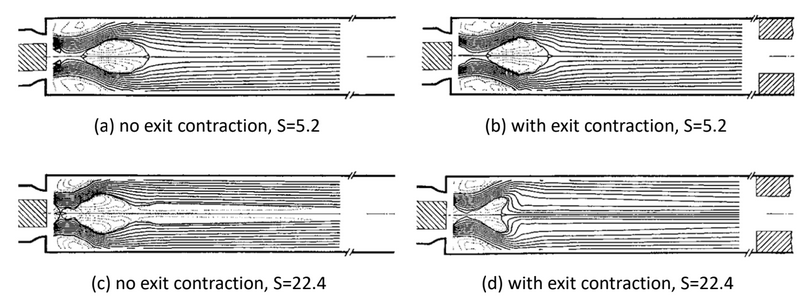
\includegraphics[width = \textwidth]{gfx/UpstreamInfluence}
\caption{Effetti di variazioni successive della geometria per un flusso vorticoso in un bruciatore}
\label{fig:UpstreamInfluence}
\end{figure}

La presenza di vortici in un passaggio divergente promuove l'esistenza di zone di ristagno e flusso inverso vicino all'asse di simmetria.
Per esempio nelle turbine a gas, questo tipo di ricircolo è incoraggiato per mantenere la stabilità della fiamma, garantendo la permanenza del fluido in una data regione per migliorare la combustione della miscela.

Per caratterizzare il livello di vortice viene definito un numero $S_w$ che altro non è che il rapporto tra il momento angolare sul raggio per il flusso assiale del momento assiale.
\begin{equation}
S_w = \frac{\int_0^{r_0}{r^2 V_{\theta}V_z dr}}{r_0 \int_0^{r_0}{r \left[V_z^2 + \left(\frac{p - p_{max}}{\rho}\right) \right]dr}}
\end{equation}
In generale si assume che 
\begin{description}
\item[$S_w < 0.5$] vortice debole o moderato
\item[$S_w > 0.5$] flusso vorticoso
\end{description}

\begin{figure}
\centering
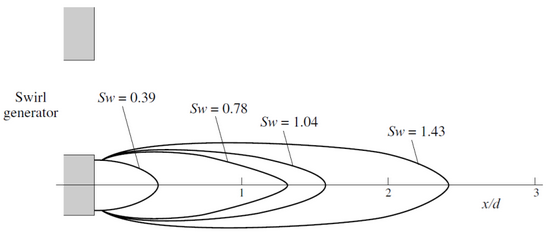
\includegraphics[width = \textwidth]{gfx/Swirl}
\caption{Esempio di misure dei vortici per un bruciatore}
\label{fig:Swirl}
\end{figure}

%%%%%%%%%%%%%%%%%%%%%%%%%%%%%%%%%%%%%%%%%%%%%%%%%%%%%%%%%%%%%%%%%%%%%%%%%%%%%%%
\chapter{Strato limite e flusso su corpi}\label{chp:BoundaryLayer}
%%%%%%%%%%%%%%%%%%%%%%%%%%%%%%%%%%%%%%%%%%%%%%%%%%%%%%%%%%%%%%%%%%%%%%%%%%%%%%%
Il concetto di strato limite nell'equazione di Navier-Stockes \eqref{eqn:NavierStockes} a pagina \pageref{eqn:NavierStockes} si può trascurare:
\begin{itemize}
\item In regioni di flusso ad alto numero di Reynolds, dove le forze viscose possono essere trascurate rispetto a quelle d'inerzia e gravitazionali (regioni non viscose)
\item Quando la vorticosità è trascurabilmente piccola da cui si ottiene l'equazione di Eulero \eqref{eqn:Eulero}.
\end{itemize}
Ci sono delle mancanze associate all'applicazione dell'equazione di Eulero in problemi pratici, in particolare l'impossibilità di descrivere condizioni di non scorrimento sulle pareti. Ne risulterebbe una descrizione irreale.

\eng{Prandtl} introdusse il concetto di:
\begin{enumerate}
\item una regione esterna considerabile come non viscida e irrotazionale.
\item uno strato limite dove il flusso deve essere considerato viscoso e rotazionale.
\end{enumerate}
Questo approccio permette di risolvere il flusso esterno considerandolo non viscido e irrotazionale, applicando l'equazione di Eulero.
Dopodiché, si usano le \textbf{condizioni dello strato limite} per legare le due regioni.
L'approssimazione dello strato limite corregge le differenze più evidenti delle equazioni di Eulero proponendo un metodo per marcare la condizione di non strisciamento sulla parete solida.

Ad oggi, nella simulazione \ac{CFD} si può anche non usare tale condizione, visto che viene già considerata in altri modelli di risoluzione del fluido.

\section{Spessore dello strato limite}
\graffito{In una data posizione in $x$, il più alto numero di Reynolds $Re_x = \frac{\rho Vx}{\mu}$ il più fino è lo strato limite e più affidabile l'approssimazione dello strato limite.}
Considerando un flusso libero ad una velocità $V$, che scorre parallelamente ad una piastra fina, semi-infinita allineata all'asse $x$.
Allora lo spessore dello strato limite $\delta = \delta(x)$, per convezione è definita come la distanza dalla parete fino alla componente di velocità parallela alla parete al $99\%$ della velocità del flusso fuori dallo strato limite.

Si può dimostrare che, per una lastra fina, infinitamente lunga:
\begin{equation}
\frac{\delta}{x} \approx \frac{1}{\sqrt{Re_x}} \Rightarrow \delta \approx \sqrt{x}
\end{equation}
\graffito{Nelle turbomacchine, il numero di Reynolds si attesta attorno a $10^5$, lo strato limite è molto più piccolo rispetto alla dimensione del canale.}

Lo sviluppo dello strato limite è, come accennato in precedenza, funzione della posizione $x$ e del numero di Reynods $Re_x$ lungo $x$.
In figura \ref{fig:BoundaryLayer} si mostra la relazione tra i due parametri.
Ingengeristicamente parlando si assume che il punto critico per il passaggio tra flusso laminare e turbolento viene ipotizzato per $Re_{x_{cr}} = 5*10^5$.

Nella pratica la transizione a flusso turbolento puà avvenire anche a valori minori di $Re_{x_{cr}}$. Ciò è influenzato dalla rugosità delle pareti solide, dalla geometria e particolari gradienti di pressione lungo la superficie.
Anche nelle simulazioni \ac{CFD} non è facile predire il valore di transizione.
Eventualmente, vengono inseriti dei dispositivi appositi per sviluppare totalmente il flusso turbolento.

\begin{figure}
\centering
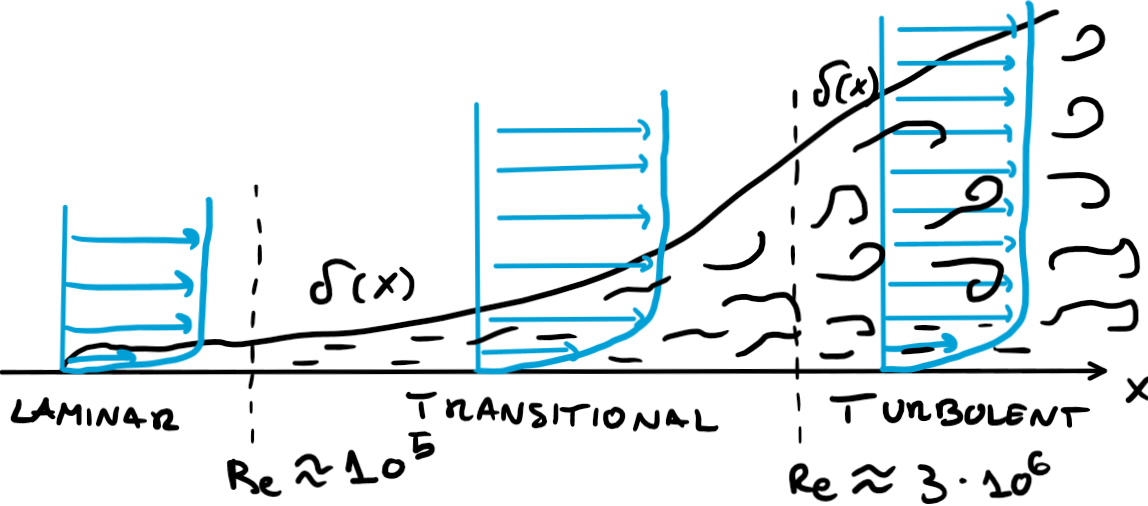
\includegraphics[width = \textwidth]{gfx/BoundaryLayer}
\caption{Sviluppo dello strato limite in funzione della distanza e del numero di Reynolds}
\label{fig:BoundaryLayer}
\end{figure}

\paragraph{Flussi liberi da ostacoli} L'approssimazione dello strato limite può essere applicata a flussi senza ostacoli come getti, scie e flussi misti.
Infatti garantiscono comunque un numero di Reynolds abbastanza alto da considerare la regione molto fina.
Le regioni di questi flussi, con viscosità non trascurabile e velocità finite, possono essere considerati come strati limite anche se non è presene una parete solida.

\section{Equazioni dello strato limite}
Consideriamo un flusso stazionario, incomprimibile planare sopra un corpo.
Si trascureranno gli effetti della gravità dato che non si sta considerando il caso di flussi liberi da superfici o convezione libera dove la gravità ha effetti considerevoli.
Considereremo solo strato limite laminare.
Considerando dei riferimenti locali nello strato limite:
\begin{itemize}
\item $x$ è parallela ovunque alla superficie e tipicamente posta a zero nel punto di stagnazione frontale del corpo. 
\item $y$ è ovunque normale al corpo.
\end{itemize}

\begin{figure}
\centering
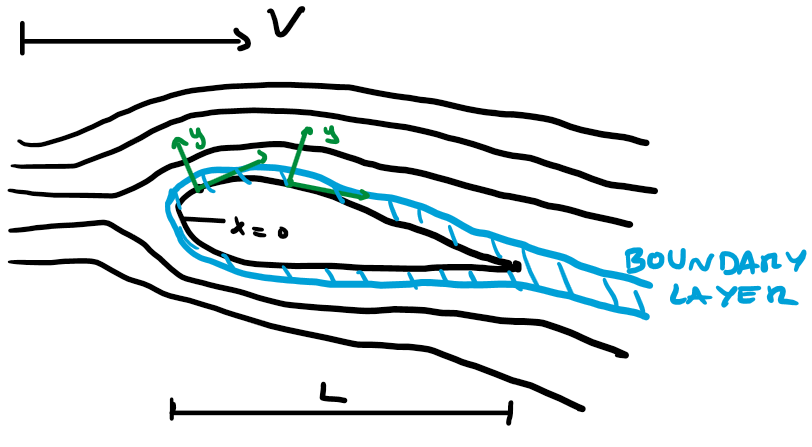
\includegraphics[width = \textwidth]{gfx/BoundaryEquation}
\caption{Riferimento per descrivere le equazioni dello strato limite}
\label{fig:BoundaryEquation}
\end{figure}

Nello strato limite, evidenziato nella figura \ref{fig:BoundaryLayer}, la componente velocità $V_y$ è molto più piccola di quella $V_x$.
$V_x \approx U$ e $V_y \approx U \frac{\delta}{L}$.

La pressione può variare lungo lo strato limite in $x$, ma il cambiamento di pressione lungo $y$ è trascurabile.
La pressione della regione esterna può essere misurata sperimentalmente da un sensore di pressione statica anche direttamente dentro lo strato limite%
\footnote{Vedi \href{https://it.wikipedia.org/wiki/Tubo_di_Pitot}{Sonda di Pitot}}.

Allora le equazioni per un flusso statico, incomprimibile, laminare nello strato limite sono:
\begin{equation}
\frac{\partial V_x}{\partial x} + \frac{\partial V_y}{\partial y} = 0
\end{equation}
Da cui:
\begin{equation}
V_x \frac{\partial V_x}{\partial x} + V_y \frac{\partial V_x}{\partial y} =%
-\frac{1}{\rho} \frac{d p}{dx} + \nu\frac{\partial^2 V_x}{\partial y^2}
\end{equation}
Infine:
\begin{equation}
-\frac{1}{\rho} \frac{dp}{dx} = U \frac{dU}{dx}
\end{equation}

\subsection{Limiti dell'equazione dello strato limite}
\begin{itemize}
\item Nel caso il numero di Reynolds non sia troppo alto, l'approssimazione dello strato limite fallisce.
\item L'assunzione che il gradiente di pressione lungo $y$ sia nullo (o quasi) non è vero nel caso in cui lo spessore dello strato limite $\delta$ è confrontabile col raggio di curvatura locale $R$. In questo caso l'accelerazione centripeta sulle \eng{streamlines} non può essere ignorata.
\item Quando il numero di Reynolds è troppo alto, allora il flusso sullo strato limite non può essere più considerato laminare. L'equazione funziona bene solamente per un flusso limite laminare.
\item In caso di separazione del flusso, l'approssimazione non è appropriata per descrivere il fenomeno nella regione di flusso separata considerato il fatto che in quel caso sono presente dei flussi di ritorno.
\end{itemize}

Le \eng{streamlines} che stanno all'interno e all'esterno dello strato limite vengono leggermente piegate lontano dalla parete col fine di garantire la conservazione della massa. Allora lo strato limite si inspessisce (esiste una componente $V_y$ piccola e finita). Anche il flusso esterno viene modificato da tali deformazioni.
Tre definizioni dello spessore dello strato limite sono state trova e attualmente utilizzate per la sua descrizione:
\begin{enumerate}
\item Lo sviluppo dello spessore
\item Il momento dello spessore
\item L'energia cinetica dello spessore.
\end{enumerate}

\subsection{Spessore dello strato limite}
\paragraph{Sviluppo dello spessore}
Possiamo descrivere lo sviluppo dello spessore attraverso la definizione:
\graffito{L'integrazione viene presa più grande rispetto a quanto richiederebbe $\delta^*$, siccome non si può conoscere lo spessore a prescindere. Comunque il contributo al integrale nella regione esterna sarebbe nulla o quasi.}
\begin{equation}
\delta^* = \int_0^{y'}\left(1-\frac{V_x}{U}\right)\,dy
\end{equation}
Allora $\delta^*$ rappresenta la distanza alla quale la parete potrebbe essere spostata in direzione normale, nel caso in cui in un ipotetico flusso uniforme non viscoso a velocità $U$ mantenga la portata nell'attuale flusso viscoso.
Può essere vista anche come un ostacolo al flusso sulla parete.

\paragraph{Momento dello spessore}
Definito come:
\begin{equation}
\theta = \int_0^{y'}{\frac{V_x}{U}\left(1-\frac{V_x}{U}\right)\,dy}
\end{equation}
$\theta$ misura la differenza tra il momento lungo tutto il flusso del flusso attuale e un flusso uniforme avente la velocità $U$ all'infuori dello strato limite.
Il momento dello spessore è fortemente legato al \eng{drag}.

\paragraph{Energia cinetica dello spessore}
\begin{equation}
\theta^* = \int_0^{y'}{\frac{V_x}{U}\left(1-\frac{V_x^2}{U^2}\right)\,dy}
\end{equation}
$\theta^*$ rappresenta la differenza tra l'energia cinetica lungo tutto il flusso attuale e quella di un flusso uniforme alla velocità $U$ all'infuori dello strato limite.
Questa rappresenta le perdine di energia cinetica per le macchine a flusso interno.

Tutti e tre i parametri $\delta^*$, $\theta$ e $\theta^*$ forniscono una misura delle defezioni di massa, momento e energia cinetica attribuite allo strato limite.

\subsection{Strato limite laminare su lastra piana}
Allora, lo strato limite su una lastra piana è spesso chiamato come \textit{a gradiente di pressione nullo}.
\textbf{Soluzione di Blasius}:
\begin{equation}
\frac{\delta}{x} = \frac{4.91}{\sqrt{Re_x}}
\end{equation}
L'approssimazione dello strato limite non è appropriata per gli spigoli della lastra perché $\delta$ non è piccolo a confronto con $x$.
Inoltre, qualsiasi lastra reale ha uno spessore finito ed è presente un punto di stagnazione sul fronte della lastra.
Si può ignorare la regione molto prossima a $x=0$ senza perdita di accuratezza per il resto del flusso.
Inoltre:
\begin{description}
\item[Sviluppo dello spessore] 
\begin{equation}
\frac{\delta^*}{x} = \frac{1.72}{\sqrt{Re_x}}
\end{equation}
\item[Momento dello spessore]
\begin{equation}
\frac{\theta}{x} = \frac{0.664}{\sqrt{Re_x}}
\end{equation}
\end{description}
Per il flusso in questione è sempre dimostrato che $\delta^*$ e $\theta$ è approssimativamente si dividono, rispettivamente, $\delta$ come $35.0\%$ e $13.5\%$ in ogni posizione di $x$.

\subsection{Strato limite turbolento su lastra piana}
Un'importante caratteristica per uno strato limite turbolento è dato dalla differenza tra i diversi strati interni dello strato limite: \eng{Inner layer} e \eng{Outer layer}.

Il profilo di velocità nell'\eng{Inner layer} dipende dalla viscosità, mentre nell'\eng{Outer layer} dipende dagli sforzi di Reynolds.
Da un'analisi dimensionale, un legame adimensionale per la velocità nell'\eng{Inner layer} è
\begin{equation}
\frac{V_x}{u_{\tau}}= f(\frac{y u_{\tau}}{v})
\end{equation}
Dove il parametro $u_{\tau}$ detto come velocità di frizione viene usato per normalizzare sia $y$ che $V_x$:
\begin{equation}
u_{\tau} = \sqrt{\frac{\tau_W}{\rho}} \qquad \tau_W = \mu\frac{\partial V_x}{\partial y}\Big|_{y=0}
\end{equation}

Variabili \eng{Inner layer}:
\begin{equation}
y^+ = \frac{y u_{\tau}}{v} \qquad u^+ = \frac{V_x}{u_{\tau}}
\end{equation}
Nell'\eng{Inner layer}: $u^+ = f(y^+)$.
La distanza non dimensionale $y^+$ è un tipo di numero di Reynolds.

\begin{figure}
\centering
\subfloat[][\emph{Suddivisione dello strato limite}\label{fig:StratoLimite}]
{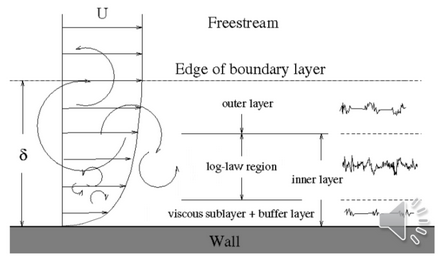
\includegraphics[width = \textwidth]{gfx/StratoLimite}}\\
\subfloat[][\emph{Leggi nello strato limite}\label{fig:LeggiStratoLimite}]
{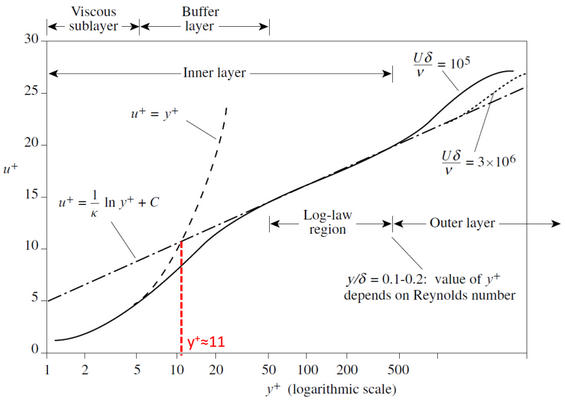
\includegraphics[width = \textwidth]{gfx/LeggiStratoLimite}}
\caption{Strato limite turbolento su lastra piana}
\label{fig:StratoLimiteTurb}
\end{figure}